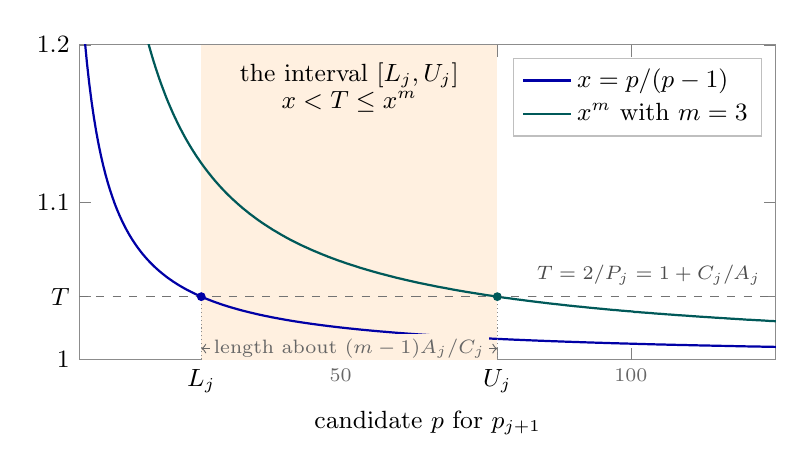
\begin{tikzpicture}
\begin{axis}[width=0.86\textwidth, height=0.46\textwidth,
  xmin=5, xmax=125, ymin=1, ymax=1.2, domain=5.5:125, samples=300,
  restrict y to domain=0.9:1.3,
  xtick={26,77}, xticklabels={$L_j$,$U_j$},
  extra x ticks={50,100}, extra x tick labels={$50$,$100$},
  extra x tick style={tick label style={font=\scriptsize, black!60}},
  ytick={1,1.04,1.1,1.2}, yticklabels={$1$,$T$,$1.1$,$1.2$},
  tick label style={font=\small}, label style={font=\small},
  xlabel={candidate $p$ for $p_{j+1}$},
  axis line style={black!45}, grid=none,
  legend style={at={(0.98,0.96)}, anchor=north east, draw=black!25, fill=white, font=\small},
  legend cell align=left]
\fill[orange!12] (axis cs:26,1) rectangle (axis cs:77,1.2);
\addplot[thick, blue!65!black] {x/(x-1)};
\addlegendentry{$x=p/(p-1)$}
\addplot[thick, teal!70!black] {(x/(x-1))^3};
\addlegendentry{$x^m$ with $m=3$}
\addplot[black!55, dashed, domain=5:125, forget plot] {1.04};
\draw[black!45, densely dotted] (axis cs:26,1) -- (axis cs:26,1.04);
\draw[black!45, densely dotted] (axis cs:77,1) -- (axis cs:77,1.04);
\fill[blue!65!black] (axis cs:26,1.04) circle (1.6pt);
\fill[teal!70!black] (axis cs:77,1.04) circle (1.6pt);
\node[font=\small, anchor=north, align=center] at (axis cs:51.5,1.195) {the interval $[L_j,U_j]$\\[-1pt] $x<T\le x^m$};
\node[font=\scriptsize, black!70, anchor=south east] at (axis cs:124,1.041) {$T=2/P_j=1+C_j/A_j$};
\draw[<->, black!60] (axis cs:26,1.007) -- node[fill=orange!12, font=\scriptsize, inner sep=1.5pt] {length about $(m-1)A_j/C_j$} (axis cs:77,1.007);
\end{axis}
\end{tikzpicture}
